
\documentclass{eecslides}

% \usecolortheme{RimouskiDark}

\usepackage[english]{babel}
\usepackage{lipsum}
\usepackage{graphicx}
\usepackage{caption}
\usepackage{hyperref}
\usepackage{xcolor}
\usepackage[protrusion=true,expansion=true]{microtype}

\title[Data Storage]{Data conservation - Perspectives, issues and solutions.}
\author[M. Bryant and S. Vissault]{\color{white}  Miranda Bryant and Steve Vissault}
\website{\color{white} s.vissault@yahoo.fr}
\institute[\color{white} UQAR]{\color{white} \textbf{Les midis numériques}}
\date{ \color{white} \today}

\setbeamersize{text margin left=1cm} 
\setbeamersize{text margin right=1cm} 
\setbeamersize{text margin top=0.1cm} 

\begin{document}



\begin{frame}[plain]
\titlepage
\end{frame}


%%%%%%%%%%%%%%%%
\section{Introduction}
%%%%%%%%%%%%%%%%

\begin{frame}{Introduction}{Context}

All biologists collect data during their career but most of them are using \alert{inapropriate files} to long term storage:

\begin{itemize}
	\item  Open Office or Microsoft spreadsheet
	\item  text and CSV files
\end{itemize}

\textbf{Some risks attributes at those practices:} Overwriting file, lost the full dataset or some records.

\end{frame}

%%%%%%%%%%%%%%%%%%%%%%%%%%%%%%%%%%%%%%%%%%%%%%%%%%%%%%%%

\begin{frame}{Introduction}{Context}

\textbf{We need to keep in mind and include those points as a part of our biologist culture:}
	
	\begin{itemize}
		\item \alert{All datasets} containing specific information given a time and a location \alert{are usefull}.
		\item Most datasets are built on \alert{public funding} and should be accessible publicly
		\item All datasets could be re-used, recycle or valorize (as the 3-R in waste management) 
	\end{itemize}


\end{frame}

%%%%%%%%%%%%%%%%%%%%%%%%%%%%%%%%%%%%%%%%%%%%%%%%%%%%%%%%

\begin{frame}{Introduction}{Why do something different ?}

\textbf{\alert{Inconvenients of spreadsheet}}

\begin{enumerate}
	\item 
\end{enumerate}

\end{frame}

%%%%%%%%%%%%%%%%%%%%%%%%%%%%%%%%%%%%%%%%%%%%%%%%%%%%%%%%


\begin{frame}{Introduction}{Why do something different ?}

\begin{figure}
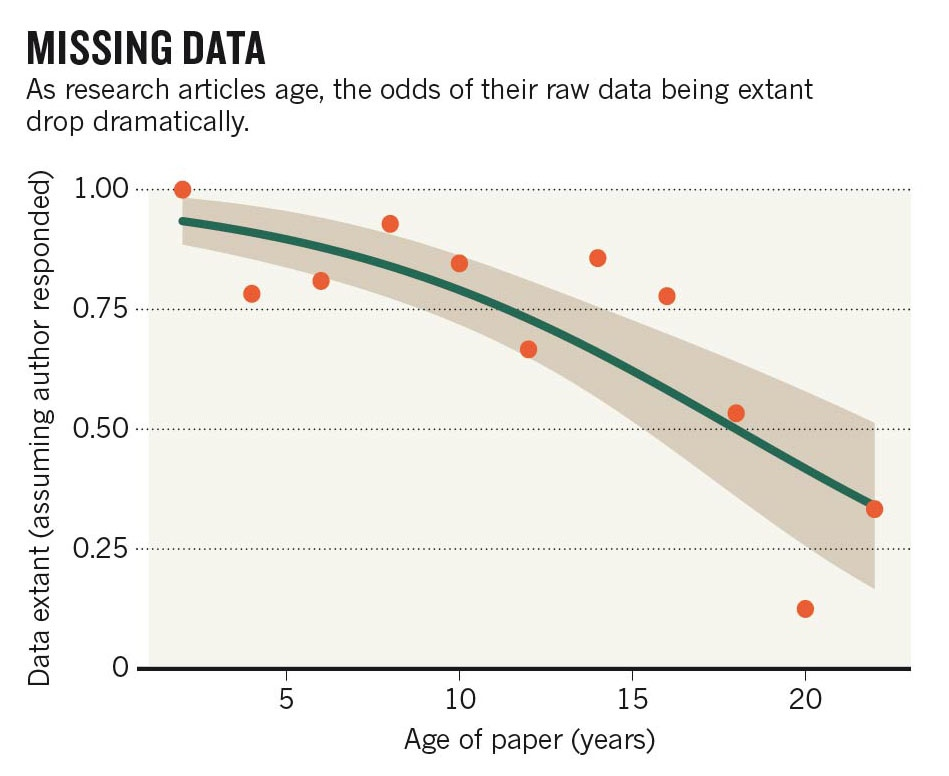
\includegraphics[width=0.65\paperwidth]{Nature_fig.jpg}
\end{figure}

\end{frame}


%\section{Références}

%	\nocite{Drever2006}
%	\nocite{Holling1973}
%	\nocite{Grenon2010}


%\begin{frame}[allowsframebreaks]{Référence}
%	\bibliographystyle{abbrv}
%	\bibliography{/home/steve/Dropbox/Bibtex/Resilience}	
%\end{frame}

\end{document}